\documentclass[UTF8]{ctexart}
\usepackage{subfiles}  

%下面的语句, 引入你的头部设置文件
\usepackage{C:/phpStorm_proj/02_myself_ID_EGO/+100_latex_all_math_sel/myPreamble} 
%必须是绝对路径,才能让各个tex在单独编译时使用到

\title{方法论}


%---------------------------------


\begin{document}
\tableofcontents % 生成目录
\date{} % 若不写这句, 则默认也会渲染出日期, 所以我们要手动赋空值
\maketitle  %这行代码, 让你前面的 title, author, date生效



\section{生活中, 哪些地方要用到线性代数?}

- 经济学研究, 经济模型通常都是线性的. \\
- 管理学中, 运筹学的一个重要议题, 是``线性规划"。许多重要的管理决策, 就是在``线性规划模型"的基础上做出的. \\
- 工程领域中更多. 飞行器设计,就要研究飞机表面气流作用的过程,包含反复求解大型的线性方程组.\\
- 马尔科夫链, 在许多学科(如生物学、商业、化学、工程学及物理学等)领域中, 被用来做数学模型. 实际上, 马尔科夫链是由一个``随机变量矩阵"所决定的一个``概率向量序列". \\
- 3D游戏, 就是以图形的``数学矩阵运算", 为基础. \\

\textbf{``线性代数"的概念和应用范围, 几乎可以涵盖所有的``自然科学"和``工程技术"领域。如果我们仍然坚持像当今的国内教学大纲做法一样, 只是把它作为计算工具进行练习,显然只是捡到了几粒芝麻 (而且如果没有掌握如MATLAB一类的软件的应用,我们捡到的是几粒陈谷子烂芝麻)! 如果要真正地弄清楚``线性代数"的应用,就必须充分了解所要应用的领域内的知识,最好有实际的工程应用的经验在里面.} 所以, 掌握线性代数的广泛应用案例、掌握线性代数的几何及物理意义、掌握线性代数的矩阵工具, 才是掌握线代的必由之路! \\




\section{几何意义 和 物理意义, 本质上是一回事}

一旦碰到较抽象难懂的新概念或定理, 如何搞定? +
- 看推导过程. +
- 弄懂它的几何意义, 或物理意义. 几何上说得通,物理上也就说得通,因为几何意义和物理意义本质上是一回事. 因为物理决定着几何结构的存在. n亿年过去了, 不符合物理规律的物质几何空间早就灭亡了. 数学家和物理学家所研究的,只是一头大象的不同部分. 


\section{真理总是简单的和直观的}

真理总是简单的和直观的. 不管多么复杂高深的数学理论,总有其直观的中心思想. 在数学中再没有别的什么东西,能比几何图形更容易进入人们的脑海了.  +
数学教育家波利亚曾经说: 一个长的证明常常取决于一个中心思想,而这个思想本身却是直观的和简单的.

事实上, 很多数学家都是先利用几何直观, 猜测到某些结果, 然后才补出逻辑上的证明的.+ 
华罗庚说过: "数缺形"时少直观, "形少数"时难入微; "数形结合"百般好, 割裂分家万事休. +
抽象和形象是相辅相成,缺一不可的.\\


\section{``线性"问题 and ``非线性"问题}

我们常说的``一次方程"和``一次函数",都属于``线性方程 Linear Equation" 和 ``线性函数 Linear Function. \\
\textbf{现实生活中的数学问题, 无非分为两类: 一类线性问题,一类非线性问题.} 线性问题是研究最久、理论最完善的. 而\textbf{``非线性问题", 则可以在一定基础上转化为``线性问题"来求解.  比如, 微积分学的基本思想, 就是``以直代曲",局部地以``切线"代替``曲线".} 于是,在某种条件下,微分方程就可以近似地变成``线性代数方程组".\\

因此, 你在遇到一个具体问题时, 首先要判断它是``线性"还是``非线性"的. 其次, 若是``非线性问题", 就考虑应如何转化为``线性问题"来解决. \\

~\\
\hrule
~\\


\section{不过原点的直线, 不满足线性代数里, 对线性函数的``比例性"的要求}

线性代数里面的``线性", 主要意思就是线性空间里的``线性变换"(映射, 类似函数的概念, 把输入变成另一种输出).\\

函数 f(x)= kx+b (k,b 是不变量),称为一元线性函数. 如果 b=0, 则这个函数的外观就变成 f(x)= k的形式了,这是一条过原点的直线.\\

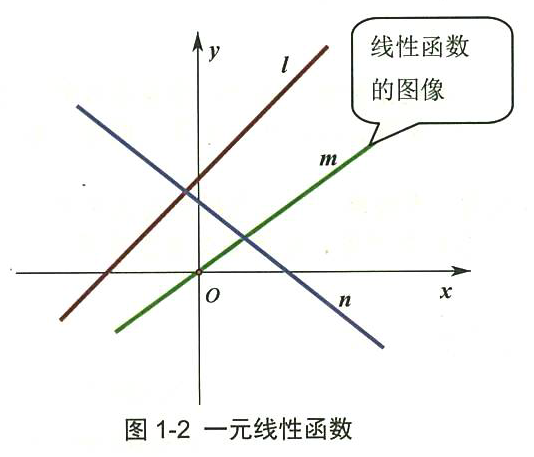
\includegraphics[width=0.4\textwidth]{img/0111.png}\\

严格说来,只有过``原点"的最简单的直线 f(x) = kx, 才被称为一元线性函数.\\

因为\textbf{虽然 f(x)=kx+b 是线性函数, 但它却不满足``线性代数"里所指的``线性"含义. 因为不过原点的直线, 不满足线性代数里, 对线性函数的``比例性"的要求.}\\

\textbf{线性函数, 其几何意义是: 它表示为一条直线. 那么其代数意义呢? 最基本的意义只有两条: ``可加性"和``比例性". }\\

【可加性】:\\
即: 如果函数 f(x) 是线性的, 则有:
\begin{align*}
	\boxed{
	f\left( x_1+x_2 \right) =f\left( x_1 \right) +f\left( x_2 \right)	
	}
\end{align*}

\textbf{其意思就是一句话: 和后的函数, 等于函数后的和.} \\
\textbf{物理意义就是说: 因变量``叠加后"的作用结果, 就等于各个因变量``独自作用结果"的叠加. 即: 先结合, 再做函数变形. 等于 先各自做函数变形, 再结合.}\\


【比例性(数乘)】:\\
也叫做齐次性、数乘性, 或均匀性. 即: 如果函数 f(x) 是线性的, 则有:
\begin{align*}
	\boxed{
	f(kx) = k \cdot f(x)	
	}
\end{align*}

一句话: \textbf{先做比例变化, 后做函数变换, 等于先做函数变换,后做比例变化.}\\
\textbf{物理意义是说: 对因变量做缩放时,函数对因变量的作用结果, 也会同等比例地缩放.} \\

\textbf{而对于不经过原点的直线 f(x)=ax+b 而言, 就不满足此``比例性".} 因为: $f(kx) = akx+b$, 而$k\cdot f(x)=akx+kb$, 所以 $f(kx) \neq k \cdot f(x)$. 因此严格地讲, f(x)=ax+b 不能再叫``线性函数"了. \textbf{或者说,线性代数的``线性变换", 不直接研究坐标系的移动.}\\

可加性与比例性组合在一块, 就是``线性"的全部意义了. 即有:
\begin{align*}
f\left( k_1x_1+k_2x_2 \right) =k_1f\left( x_1 \right) +k_2f\left( x_2 \right) \ \ ←\ k_1,k_2\text{为常数}
\end{align*}
\textbf{一句话: 线性组合的函数,等于函数的线性组合。}这里面既有``缩放"又有``叠加"的物理含义.\\

在物理上, 线性函数的\textbf{``可加性"表明: 函数所描述的事物, 具有累加性. 即: 所有起因的累加, 所导致的结果, 完全等于``每个起因独自所引起的结果"的累加。}\\
\textbf{是否满足``可加性", 就界定了它所描述的事物, 到底是``线性"的, 还是``非线性"的.}\\


比例性是啥物理含义呢? \textbf{比例性又名``齐次性", 说明没有初始值。没有输入信号时, 输出也没有; 有几倍的输入量, 就刚好就有几倍的输出量.}


~\\
\hrule
~\\


\section{y=Kx 所做的动作, 就是将一个向量x, 通过矩阵K, 映射变换为另一个新向量y. 矩阵K, 就相当于一个``函数"的作用.}

$
\left\{ \begin{array}{l}
	y_1=k_{11}x_1+k_{12}x_2+...+k_{1n}x_n\\
	y_2=k_{21}x_1+k_{22}x_2+...+k_{2n}x_n\\
	...\\
	y_m=k_{m1}x_1+k_{m2}x_2+...+k_{mn}x_n\\
\end{array} \right. \ ←k_{11},...,k_{mn}\ \text{不是变量,而是系数}
$\\

如上式, 这m个n维(n元)线性函数, 都是齐次函数. 他们全部过原点. \\
线性齐次函数, 形如 $	y=k_{1}x_1+k_{2}x_2+...+k_{n}x_n$, \textbf{这个式子中, 每项里的变量x出现的次数, 都是一次的(没有常数项),整齐划一,故此称为``齐次"的.} 全称为``n元线性齐次函数". \\

上式, 可等价写成: 
$
\left| \begin{array}{l}
	y_1\\
	y_2\\
	...\\
	y_m\\
\end{array} \right|=\left[ \begin{matrix}{l}
	k_{11}&		...&		&		k_{1n}\\
	...&		&		&		\\
	&		&		&		\\
	k_{m1}&		&		&		k_{mn}\\
\end{matrix} \right] \left| \begin{array}{l}
	x_1\\
	x_2\\
	...\\
	x_n\\
\end{array} \right|
$ \\

并可进一步简写成: y=f(x) = Kx \\
即:
$
y=\left| \begin{array}{l}
	y_1\\
	y_2\\
	...\\
	y_n\\
\end{array} \right|,\ K=\left[ \begin{matrix}
	k_{11}&		...&		&		k_{1n}\\
	...&		&		&		\\
	&		&		&		\\
	k_{m1}&		&		&		k_{mn}\\
\end{matrix} \right] ,\ x=\left| \begin{array}{l}
	x_1\\
	x_2\\
	...\\
	x_n\\
\end{array} \right|
$\\
\vspace{1em} 

\textbf{矩阵, 其实就是线性方程组的``系数". 矩阵, 就核心地代表了``线性变换".}\\
因为 \textbf{y=Kx 所做的动作, 就是将一个向量x, 通过矩阵K, 映射变换为另一个新向量y. 矩阵K, 就相当于一个``函数"的作用. 即, 一个矩阵对应着一种``线性变换"规则.} \\

~\\
\hrule
~\\

\section{线性超平面}


f(x) = kx 是二维坐标空间中的几何图形. \\

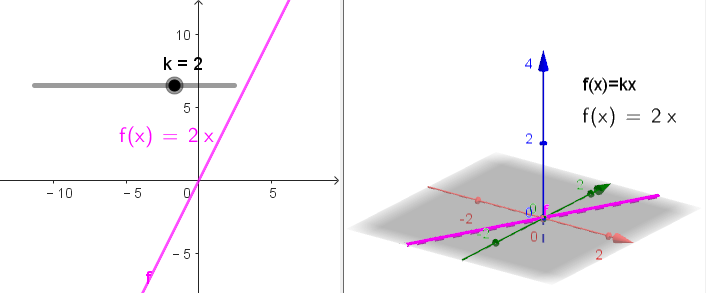
\includegraphics[width=0.8\textwidth]{img/0112.png}\\

把这个二维直线, 放到三维空间中, 其函数表达式, 就要改写成: $f\left( x_1,x_2 \right) =k_1x_1$ 或 $f\left( x_1,x_2 \right) =k_1x_2$. 它的图形是一个过原点的``平面". 其中, 多出来的这个$x_2$, 可以取任意值. 也就是说:  $f\left( x_1,x_2 \right) =k_1x_1$ 的图像, 是一个过 $x_2$坐标轴的平面. \\

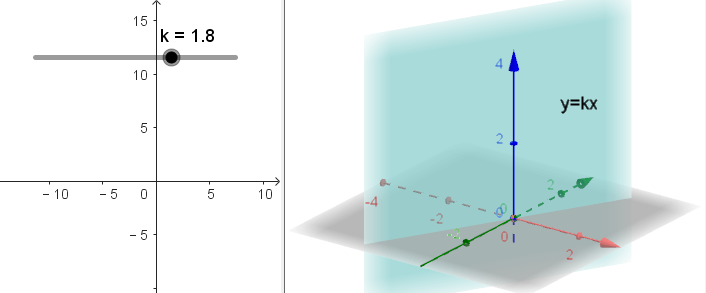
\includegraphics[width=0.8\textwidth]{img/0113.png}\\

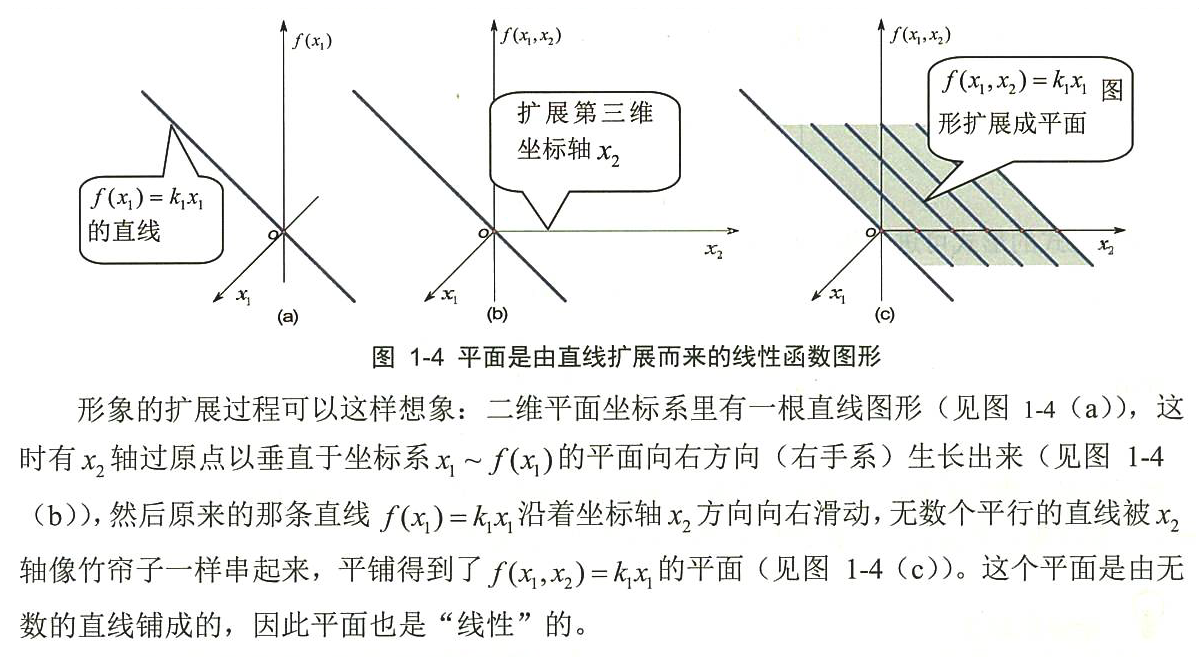
\includegraphics[width=1\textwidth]{img/0114.png}\\

既然在三维空间中, $k_1 x_1$ 是一个平面, 那么 $k_1 x_1 +  k_2 x_2$, 就是两个平面相加了. 即就是 $f\left( x_1,x_2 \right) =k_1x_1$ 和 $f\left( x_1,x_2 \right) =k_2 x_2$ 的图形相加. \textbf{一般情况下, 两个平面相加, 仍然是一个平面.} \\

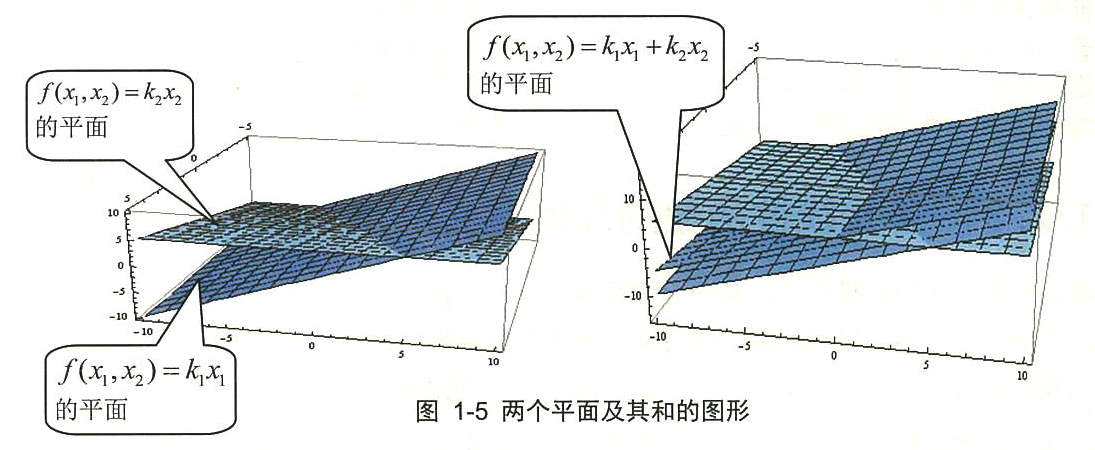
\includegraphics[width=1\textwidth]{img/0115.png}\\

因此,线性函数 $f(x_1, x_2) = k_1 x_1 + k_2 x_2$的几何图形, 是一个过原点的平面. \textbf{这个平面, 是在三维坐标系下的二维几何图形.}\\

由二元线性函数 $
f\left( x_1,x_2 \right) =k_1x_2+k_2x_2
$ 继续扩展到三元线性函数$
f\left( x_1,x_2,x_3 \right) =k_1x_2+k_2x_2+k_3x_3
$时,所在的坐标系, 由三维扩展到四维。可以想象: 这个三元变量函数, 构成了一个三维空间,是由三个空间
$f\left( x_1,x_2,x_3 \right) =k_1x_1$, 
$f\left( x_1,x_2,x_3 \right) =k_2x_2$,
$f\left( x_1,x_2,x_3 \right) =k_3x_3$ 叠加得到的. 因此它是一个四维空间中(四维坐标系)的一个三维子空间. \\

继续扩展到``四元", 及``n元"的线性函数$
f\left( x_1,x_2,...,x_n \right) =k_1x_2+k_2x_2+...+k_nx_n
$,坐标系空间扩展到五维, 乃至n+1维,\textbf{其几何图形, 仍将是一个低于坐标系维度一个维数的``子空间''.} \\

\textbf{这个n元几何图形, 总是低于坐标系一个维数。我们常常把一个高维的坐标系, 称为一个``空间''. 那么,只能把这个线性函数低一维的几何图形, 称为一个``平面''. 这是一个扩展意义上的平面,常被称为``超平面"}(原理如同 对于三维``空间里''而言,低一维度的子空间就是平面). \textbf{所以, 超平面等同于包含在n维空间$R^n$中的 n-1维 欧式空间},它们对应于通常三维空间中的二维平面、平面内的直线、直线上的点等. \\


把线性函数$
f\left( x_1,x_2,...,x_n \right) =k_1x_2+k_2x_2+...+k_nx_n
$的形式改写为 \\
$
k_1x_2+k_2x_2+...+k_nx_n-f\left( x_1,x_2,...,x_n \right) =0
$\\
或者更一般的形式为\\
$
k_1x_2+k_2x_2+...+k_nx_n+k_{n+1}x_{n+1}=c
$\\
这是一个 n+1维空间 $R^{n+1}$中的一个n维超平面,只是这个平面不一定过原点了(注意,\textbf{不过原点的超平面, 依然可称之为``空间",但不能称之为``线性空间"}). \\

\textbf{因此, 我们就明白了多元线性函数的``线性", 不能单纯地理解为空间中的一条直线了,把线性函数几何图形, 想象成一个``平面", 更有代表性。}\\
\textbf{实际上,把n个n元线性函数, 组成一个``满秩方程组", 才能表示一条直线。}\\

\textbf{相比较而言,线性函数中含有的参数少,涉及的运算简单,仅为``加法"和``乘法",便于运算,是变量数学中最简单的函数. 其实许多复杂的函数, 都可以在一定范围和精确度下, 近似地``用线性函数"来表示. 所以``线性函数"是变量数学中最重要的函数。}\\


~\\
\hrule
~\\



\section{线性映射}

\textbf{线性函数, 用运动的概念来理解, 就是``映射", 如同函数的功能一样.} \\


下面的图, 给出了一元线性齐次函数 f(x)=kx,  当``k取不同的数"时的映射对应关系。注意: 在三个分图中,有一个共性就是:元素0必然映射到元素0. \\

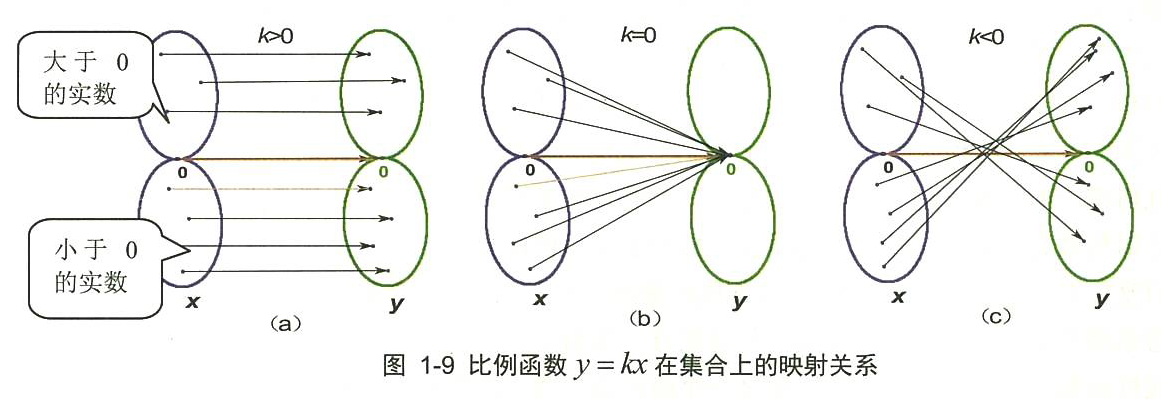
\includegraphics[width=1\textwidth]{img/0116.png} \\

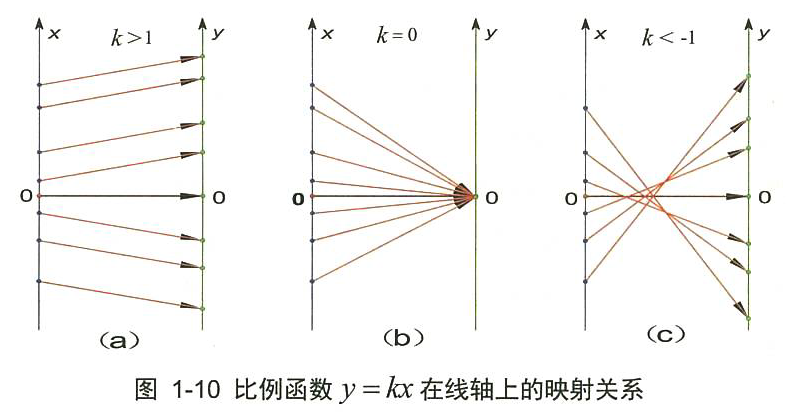
\includegraphics[width=0.7\textwidth]{img/0117.png}\\


如果把两个坐标轴的原点, 进行重合(因为0元素必然映射到0元素),再把两个坐标轴的夹角, 调整到 $\frac{\pi}{2}$角,就可得到笛卡尔平面坐标系 (而\textbf{线性代数中讲的``线性空间"坐标系的坐标轴, 可以是任意非零的夹角}). 如下图只画出 k>0 的映射情况. \\
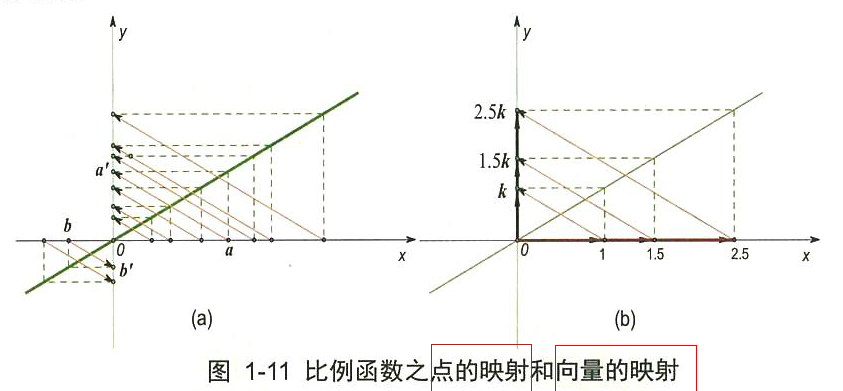
\includegraphics[width=0.7\textwidth]{img/0118.png}\\

上图, 如果把点a、a'、b和b', 分别与原点0连起来,就会得到线段 0a、0b、0a'、0b'。于是, 线段0a, 映射到线段0a'; 线段0b, 映射到线段0b'.\\
所以, 线性映射, 就是把``线段"映射到``线段". \\
如果我们把``线段"改称为``向量"的话,就是: \textbf{线性映射就是把``向量"映射成``向量"}(见图 1-11(b)). 线性映射把向量变成另外一个向量.\\

当然,这个线性映射, 也满足线性的``可加性"和``比例性"的性质: \\
→ \textbf{可加性: 两个向量先求和, 再映射. 结果就等于: 先各自映射, 再求和.} (即: x轴上的两向量的和, 映射得到的y轴向量, 等于``两个x轴向量,分别映射得到的y轴向量"的和.) \\
→ \textbf{比例性:  先倍数, 再映射. 结果就等于: 先映射, 再倍数.} (即:``x轴向量的倍数"映射得到的y轴向量, 等于``x轴向量映射的y轴向量"的倍数)(见图1-11 (b)).\\

用数学表示上面的这两种性质, 就是: \\
→ $T(a+b) = Ta + Tb$ \\
→ $T(ka) = k \cdot Ta$ \\
其中, T是映射运算(即矩阵), a、b是任意两个向量. \\

\textbf{T本来表示一种``线性映射"的动作关系(或函数关系). 但在上式中, 就像一个实数或变量一样参与运算。}如T(a+b)=Ta+Tb,就像乘法对加法的分配律一样展开运算. \textbf{因此T在这里, 也叫``线性算子"。具体的算子有: 微分算子、积分算子、拉普拉斯算子等。} \\


\begin{myEnvSample}
$
\left| \begin{array}{l}
	y_1\\
	y_2\\
\end{array} \right|=\left[ \begin{matrix}
	a_1&		a_2\\
	b_1&		b_2\\
\end{matrix} \right] \left| \begin{array}{l}
	x_1\\
	x_2\\
\end{array} \right|
$ 的几何解释是:\\
\textbf{向量x和y, 都是二维向量. 因此, 所有任意的向量x的集合, 将构成平面$\varPi _1$,所有任意的向量y的集合, 会构成平面$\varPi _2$。所以,二维线性函数, 就构成了两个二维平面之间由矩阵K所确定的映射关系.(此处, 矩阵是二维的比率).} \\

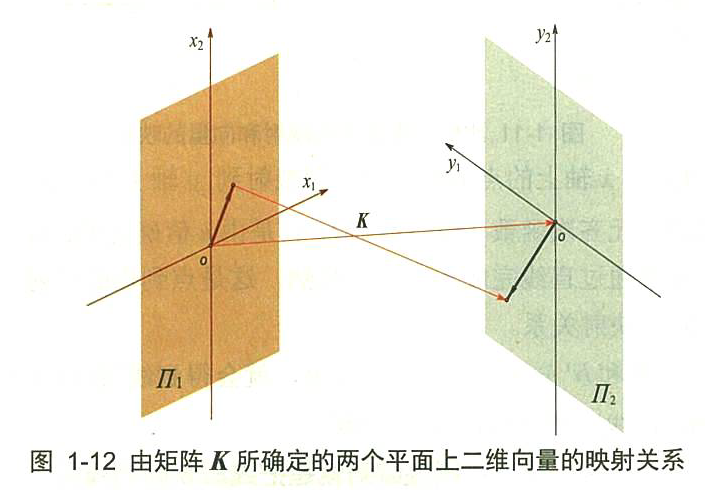
\includegraphics[width=0.6\textwidth]{img/0119.png}\\

\textbf{平面$\varPi _1$的原点0, 始终映射到另一个平面$\varPi _2$的原点0,这是``线性映射"的最基本要求。}\\

为了更仔细地观察映射之间的关系,我们把平面$\varPi _1$放平,并使两个平面的原点0重合,就得到了一个由两个相交平面, 所构造的三维空间。\\

图1-13中,把平面$\varPi _1$上的向量x, 标注为$a_i$,把平面$\varPi _2$上的向量y, 标注为$b_i$,(为了和坐标系的标注区别开来)。

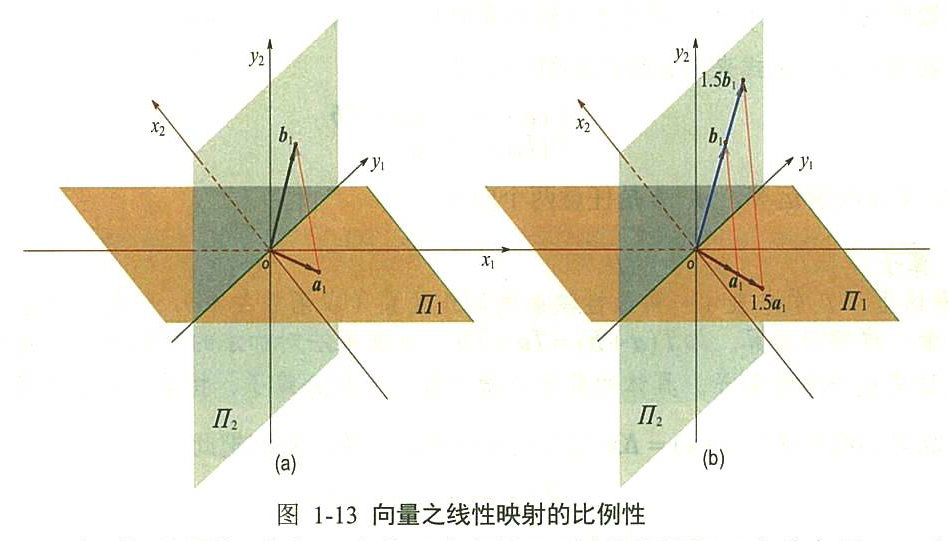
\includegraphics[width=0.8\textwidth]{img/0120.png}\\

图1-13(a)表示: 矩阵K, 把平面$\varPi _1$上的一个向量$a_1$, 映射到平面$\varPi _2$上的向量$b_1$. 也即``有向线段"映射为``有向线段". \\
图1-13(b)表示: 把一个向量$a_1$比例放大到1.5倍后, 用矩阵K的规则, 来映射到平面$\varPi _2$上的向量 $1.5b_1$. 这满足线性映射的``比例性"。\\
\end{myEnvSample}


\textbf{其实, 对于``数乘变换" T(a)= ka,除了把a看做向量外,我们可以把a看做一个几何图形(其实``向量"也是一个几何图形,只不过它是一个简单的几何图形 -- 有向线段).}\\
→ T 在 k>1时, 就是对向量线段(几何图形)a放大 \\
→ T 在 0<k<1时, 就是对a缩小 \\
→ T 在 k=-1时, 就是把a反方向变化 \\

~\\
\hrule
~\\


\section{``线性变换"的几何意义}

\textbf{在大多数的教科书中,``线性映射"和``线性变换"被区别为两个概念。\\
如果映射是发生在一个集合上的``同一个坐标系"中,``线性映射"就被称为``线性变换"。所以, ``线性变换"其实只是作为``线性映射"的特例而已},就是把集合上的两个坐标系, 合并为在一个上显示而已. \\

比如下例, 本来有两个平面 $\varPi_1$ 和 $\varPi_2$. 现在, 我们把 $\varPi_2$平面旋转后让它躺下,  让 $y_1$轴重合于$x_1$轴,$y_2$轴重合于$x_2$轴,即把两个平面合二为一了. 从左图的状态, 变成了右图的状态. 这个, 就是从``线性映射"转换成了``线性变换".\\

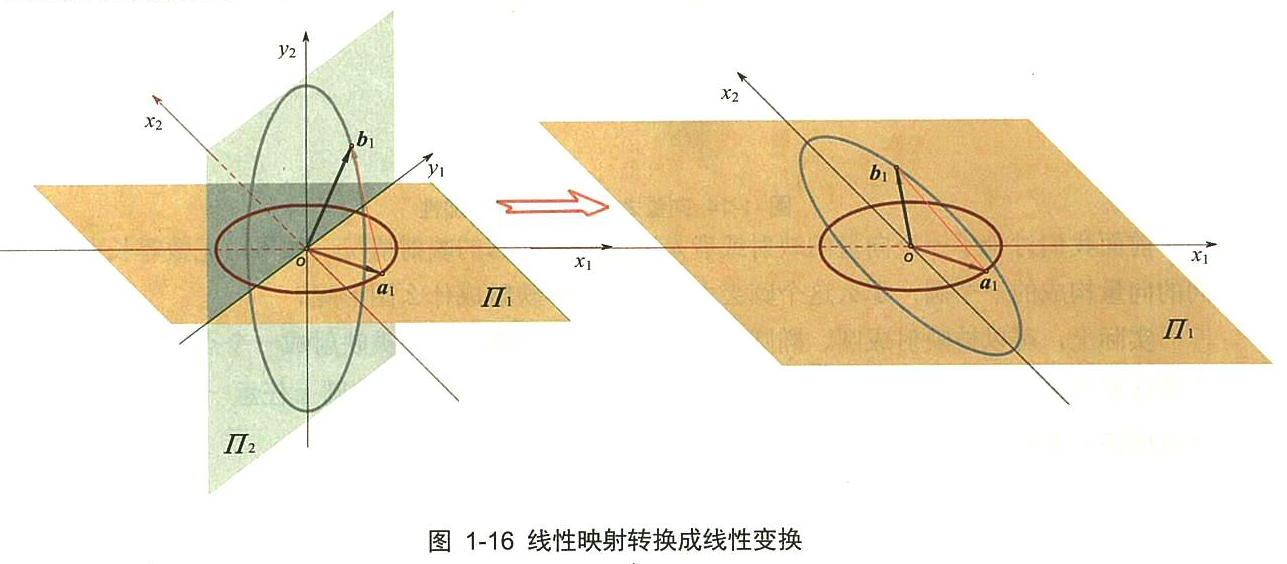
\includegraphics[width=0.8\textwidth]{img/0121.png}\\

- 可加性: 先把两个向量求和, 再做变换, 结果就等于先把这两个向量做变换, 再求和. \\
- 比例性: 将数k, 和一个向量做数乘, 然后再进行变换, 结果就等于先把这个向量做变换, 再乘以数k. \\

用公式表示, 即``线性变换"是满足这两条公式的 (T是矩阵, a,b是向量, k是倍数): \\
$T(a+b)=Ta+Tb$ \\
$T(ka) = k \cdot Ta$ \\

在工程中常用的差分运算、微分运算, 及积分运算, 都属于``线性变换",都满足以上的``可加性"和``比例性"的关系.

线性变换,可以有两个方面的含义: \\
1.对空间里的``向量", 做变换,但保持``空间坐标系"不变. \\
2.对``坐标系"做变换, 但保持``向量"不变. \\

线性代数, 是高等代数的一大分支。在研究多变量问题(多元函数)时, 如果变量间的因果关系是``线性"的,那么称这个问题为线性问题。\\

\textbf{线性问题, 或方程里的``变量", 就是``向量". 因此一说``线性"必提``向量".} \\
一般的线性代数课本里的主要内容: 行列式、向量组、矩阵、线性方程组, 及二次型等,这些内容都是对``向量"的函数或组合.

``向量"的概念,从数学的观点来看, 不过是``有序多元数组".\\
\textbf{没有掌握``线性代数", 要去学习自然科学, 简直就是文盲.} 要是没有线性代数,任何数学和初等教程都讲不下去。\\


~\\
\hrule
~\\





\end{document}